\section*{Chapter 5}

\subsection*{Exercise 5.1}

$f: \mathbb{R}^3 \to \mathbb{R}^3$. $D_f = \begin{bmatrix} 3 & 1 & 1 \\ 0 & e^yz & e^y \\ yz & xz & xy \end{bmatrix}$

\subsection*{Exercise 5.2}

\begin{minipage}{0.45\linewidth}
    \begin{center}
        \tikzsetnextfilename{c05e02-01}%
        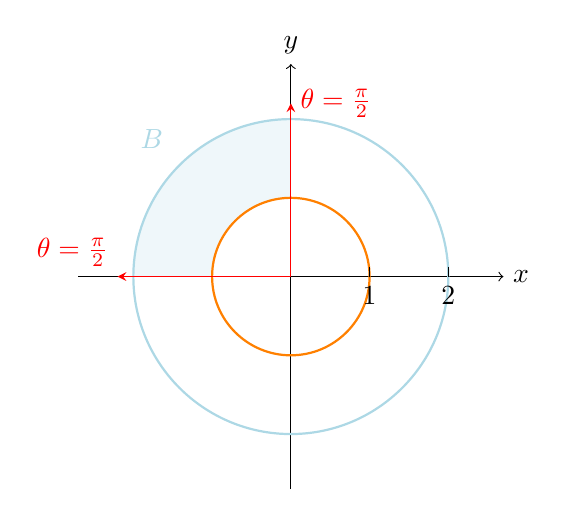
\begin{tikzpicture}
            \fill[LightBlue,fill opacity=0.2] (0,0) -- (180:2) arc (180:90:2) -- cycle;
            \fill[white,] (0,0) -- (180:1) arc (180:90:1) -- cycle;
            
            \draw[->] (-2.7,0) -- (2.7,0) node[right] {$x$};
            \draw[->] (0,-2.7) -- (0,2.7) node[above] {$y$};
            
            \draw[thick,LightBlue] (0,0) circle (2);
            \draw[thick,orange] (0,0) circle (1);
            
            \node[LightBlue,above left] at (-1.5,1.5) {$B$};
            
            \draw[red,-stealth] (0,0) -- (0,2.2) node[right] {$\theta=\frac{\pi}{2}$};
            \draw[red,-stealth] (0,0) -- (-2.2,0) node[above left] {$\theta=\frac{\pi}{2}$};
            \draw (1,0.125) -- (1,0) node[below] {$1$};
            \draw (2,0.125) -- (2,0) node[below] {$2$};
        \end{tikzpicture}
    \end{center}
\end{minipage}
$\overset{g}{\longrightarrow}$
\begin{minipage}{0.45\linewidth}
    \begin{center}
        \tikzsetnextfilename{c05e02-02}%
        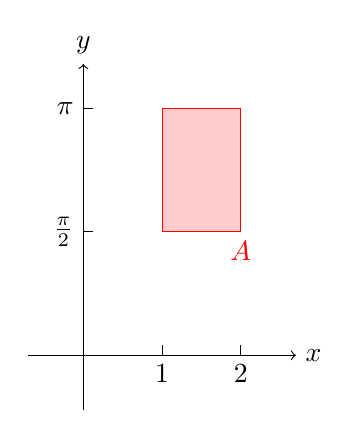
\begin{tikzpicture}
            \draw[->] (-0.7,0) -- (2.7,0) node[right] {$x$};
            \draw[->] (0,-0.7) -- (0,3.7) node[above] {$y$};
            
            \draw[red,fill=red,fill opacity=0.2] (1,1.57) -- (1,3.14) -- (2,3.14) -- (2,1.57) -- cycle;
            
            \draw (0.125,1.57) -- (0,1.57) node[left] {$\frac{\pi}{2}$};
            \draw (0.125,3.14) -- (0,3.14) node[left] {$\pi$};
            
            \draw (1,0.125) -- (1,0) node[below] {$1$};
            \draw (2,0.125) -- (2,0) node[below] {$2$};
            
            \node[red,below] at (2,1.57) {$A$};
        \end{tikzpicture}
    \end{center}
\end{minipage}

$\begin{aligned}[t]
    \int_B x
     & = \int_A x \color{red} \cdot r                                                                             \\
     & = \int_{r=1}^{r=2} \int_{\theta=\frac{\pi}{2}}^{\theta=\pi} r \cos{\theta} \cdot r \,d\theta \,dr          \\
     & = \int_{r=1}^{r=2} r^2 \left( \int_{\theta=\frac{\pi}{2}}^{\theta=\pi} \cos{\theta} \,d\theta \right) \,dr \\
     & = \left( \int_{r=1}^{r=2} r^2 \,dr \right) \cdot\left( \int_{\theta=\frac{\pi}{2}}^{\theta=\pi} \cos{\theta} \,d\theta \right) \\
     & = \frac{r^3}{3} \bigg|_1^2 \cdot \sin{\theta} \bigg|_{\frac{\pi}{2}}^\pi                                   \\
     & = -\frac{7}{3}
\end{aligned}$

\subsection*{Exercise 5.3}

\begin{proof}
$\begin{aligned}[t]
    \left( \int_{-\infty}^{\infty} e^{-x^2} \,dx \right)^2
     & = \left( \int_{-\infty}^{\infty} e^{-x^2} \,dx \right) \cdot \left( \int_{-\infty}^{\infty} e^{-x^2} \,dx \right) \\
     & = \left( \int_{-\infty}^{\infty} e^{-x^2} \,dx \right) \cdot \left( \int_{-\infty}^{\infty} e^{-y^2} \,dy \right) \\
     & = \int_{x=-\infty}^{x=\infty} \left( \int_{y=-\infty}^{y=\infty} e^{-y^2} \,dy \right) e^{-x^2} \,dx              \\
     & = \int_{x=-\infty}^{x=\infty} \int_{y=-\infty}^{y=\infty} e^{-x^2} \cdot e^{-y^2} \,dy \,dx                       \\
     & = \int_{x=-\infty}^{x=\infty} \int_{y=-\infty}^{y=\infty} e^{{-(\color{red}x^2 + y^2})} \,dy \,dx                 \\
     & = \int_{r=0}^{r=\infty} \int_{\theta=0}^{\theta=2\pi} e^{-r^2} \cdot r \,d\theta \,dr                             \\
     & = 2\pi \int_{r=0}^{r=\infty} e^{-r^2} \cdot r \,dr
\end{aligned}$

Take $\begin{cases} u = -r^2 \\ du = -2r \,dr \end{cases}$, we have $\int e^{-r^2} \cdot r = -\frac{1}{2} \int e^u \,du = -\frac{1}{2} e^{-r^2}$. 

Thus, $\begin{aligned}[t]
    2\pi \int_{r=0}^{r=\infty} e^{-r^2} \cdot r \,dr
     & = 2\pi \cdot \left( -\frac{1}{2} \right) \left( e^{-r^2} \bigg|_{0}^{\infty} \right) \\
     & = -\pi \cdot (e^{-\infty} - e^{-0^2})                                                \\
     & = \pi
\end{aligned}$

Thus, $\int_{-\infty}^\infty e^{-x^2} \,dx = \sqrt{\pi}$. 
\end{proof}

\subsection*{Exercise 5.4}

\subsection*{Exercise 5.5}

$\begin{aligned}[t]
    V & = \int_{\theta=0}^{\theta=2\pi} \int_{r=0}^{r=1} \int_{z=0}^{{z=\color{red}a(r-1)^2}} 1 \cdot r \,dz \,dr \,d\theta \\
      & = \int_{\theta=0}^{\theta=2\pi} 1 \,d\theta \cdot \int_{r=0}^{r=1}\int_{z=0}^{z=a(r-1)} r \,dz \,dr                 \\
      & = 2\pi \int_{r=0}^{r=1} r(a(r-1)^2 - 0) \,dr                                                                        \\
      & = 2\pi a \int_{r=0}^{r=1} r^3 - 2r^2 + r \,dr                                                                       \\
      & = 2\pi a \left( \frac{r^4}{4} + \frac{2r^3}{2} + \frac{r^2}{2} \right) \bigg|_{r=0}^{r=1}                           \\
      & = 2\pi a \left( \frac{1}{4} + \frac{2}{3} + \frac{1}{2} \right)                                                     \\
      & = \frac{\pi}{6} \cdot a \color{LightBlue} = 1 \implies a = \frac{6}{\pi}
\end{aligned}$

\subsection*{Exercise 5.6}

Set $x^2 + y^2 + z^2 = R^2$. Then, $\begin{aligned}[t]
    V &= \int_B 1 \,dA \\
    &= \int_{\theta=-\frac{\pi}{2}}^{\theta=\frac{\pi}{2}} {\color{DarkGreen} \int_{\rho=0}^{\rho=R} \int_{\phi=0}^{\phi=\pi}} 1 {\color{red} \cdot \rho^2 \sin(\phi) } \,d\phi \,d\rho \,d\theta
\end{aligned}$